\documentclass[11pt]{beamer}
\usepackage[UTF8,scheme=plain]{ctex}
\usepackage{listings}
\usepackage[utf8]{inputenc}
\usepackage[T1]{fontenc}
\usepackage{amsmath}
\usepackage{amsfonts}
\usepackage{amssymb}
\usepackage{graphicx}
\usetheme{Boadilla}

\usepackage{framed} % 可以用 \begin{shaded},即背景色块
\definecolor{shadecolor}{rgb}{0.9,0.9,0.9}

\newcommand{\kong}[1][0.5]{\vspace{#1cm}}

\begin{document}
	\author{ 路毅 \hspace{0.3cm} 曲阜师范大学 }
	\date{\number\year 年 \number\month 月 \number\day 日}
	\title{数学物理方法第一章}

\begin{frame}
	\maketitle
\end{frame}

\kaishu

\begin{frame}{教材与参考书}
教材:川大版 《高等数学》 第四册第三版

\kong[0.5]

参考书:
\begin{itemize}
\item 梁昆淼《数学物理方法》
\item Arfken \& Weber "Mathematical methods for physicists"
\end{itemize}

\kong[0.5]

课程交流qq群:1056754073
\end{frame}

\begin{frame}{课程内容}
\begin{itemize}
	\item 第一篇:复变函数论(1-7周)\\
		  应用:光学、量子力学、固体物理等\\
		  \vspace{0.5cm}
	\item 第二篇:数学物理方程(8-13周)\\
		  应用:电动力学、量子力学、分析力学、流体力学、计算物理等\\
		  \vspace{0.5cm}
	\item 第三篇:特殊函数(14-17周)\\
	      应用:电动力学、量子力学等\\
		  \vspace{0.5cm}
	\item 复习(18周)
\end{itemize}
\end{frame}

\begin{frame}{怎样学好数学}
1. 做练习、做练习、做练习\\
\vspace{0.5cm}
2. 思考、讨论与交流\\
\vspace{0.5cm}

每1-2周安排一次线上答疑,敬请关注。
\end{frame}

\begin{frame}{第一章:复数与复变函数}
\begin{itemize}
	\item 第一节:复数
	\vspace{1cm}
	\item 第二节:复变函数的基本概念
	\vspace{1cm}
	\item 第三节:复球面与无穷远点
\end{itemize}
\end{frame}

\begin{frame}{什么是复数}
在过去,我们认为
\begin{equation}
\sqrt{-1}
\end{equation}
是没有意义的。

所以我们解一元二次方程时,
\begin{equation}
ax^2 + bx +c = 0, (a \neq 0)
\end{equation}
得到
\begin{equation}
x = \frac{-b \pm \sqrt{b^2 - 4 ac } }{2a},
\end{equation}
我们要求
\begin{equation}
\Delta = b^2 - 4 ac \geq 0,
\end{equation}
否则认为方程无解。
\end{frame}

\begin{frame}{什么是复数}
这是因为,没有任何一个实数的平方是负数。\\

现在,我们定义$i$,
\begin{equation}
i^2 = -1,
\end{equation}

它不是一个实数,是我们新引进的概念,叫做虚数单位。
引入它以后,我们可以得到一种新的数
\begin{equation}
z = x + i y,
\end{equation}
其中,$x,y$是实数,这样定义的$z$叫做复数,相应地,$x,y$是$z$的实部和虚部,有时记作
\begin{equation}
x = Re z, y = Im z,
\end{equation}
其中$Re$是Real的缩写,即实部,$Im$是$Imaginary$(想象的,虚的)的缩写,即虚部。

例如:
\begin{equation}
3 + 5i, 2 + 4i, -1 + 2i
\end{equation}

\end{frame}

\begin{frame}{什么是复数}
\begin{equation}
z = x + i y,
\end{equation}
那么,如果$y=0$,就有$z=x$,是一个实数,所以复数包括所有实数,是实数域的推广。

\kong

如果$x=0,y\neq 0$,就有$z= yi$,这样的数叫做纯虚数。

\kong[0.5]

例如,$i$是一个纯虚数,因为
\begin{equation}
i = 0 + 1*i.
\end{equation}

\kong

请问:纯虚数的平方是什么样的数?

\end{frame}

\begin{frame}{复数相等}
如果有两个复数,
\begin{equation}
z_1 = x_1 + i y_1, z_2 = x_2 + i y_2,
\end{equation}
那么,$z_1 = z_2$当且仅当
\begin{equation}
x_1 = x_2, y_1 = y_2.
\end{equation}

例如:
\begin{equation}
1 + 2i \neq 1 + 3i,
\end{equation}
因为它们虚部不相等。
\begin{equation}
1 + 2i \neq 0 + 2i,
\end{equation}
因为它们实部不相等。
\end{frame}

\begin{frame}{复数的运算}
在实数域中,最基本的两种运算是加法和乘法,减法和除法分别是它们的逆运算。

\kong

在复数中,我们可以自然地推广加法和乘法,
若有
\begin{equation}
z_1 = x_1 + iy_1, z_2 = x_2 + i y_2,
\end{equation}
则加法为
\begin{equation}
z_1 + z_2 = (x_1 + x_2) + i(y_1 + y_2),
\end{equation}
乘法定义为
\begin{equation}
z_1 * z_2 = (x_1 + iy_1)(x_2 + iy_2) = (x_1 x_2 - y_1 y_2) + i(x_1 y_2 + x_2 y_1)
\end{equation}

\end{frame}

\begin{frame}{复数的运算}
减法是加法的逆运算
\begin{equation}
z_1 - z_2 = (x_1 - x_2) + i(y_1 - y_2),
\end{equation}
除法是乘法的逆运算,若 $z_2 \neq 0$,则
\begin{equation}
z_1 / z_2 = \frac{ x_1 + i y_1 }{ x_2 + i y_2} = \frac{ (x_1 + iy_1)(x_2 - i y_2) }{ (x_2+iy_2)(x_2 - iy_2) } = \frac{ x_1 x_2 + y_1 y_2 + i(x_2 y_1 - x_1 y_2) }{ x^2_2 + y^2_2}
\end{equation}
上面的式子采用了分式化简的手法,将分母化成实数。
\end{frame}

\begin{frame}{例题}
例如
\begin{eqnarray}
(-1 + i) + (1-i) &=& 0, \\
(-1 + i) * (1+i) &=& -2, \\
(-1 + i) / (1+i) &=& \frac{ (-1+i)(1-i) }{(1+i)(1-i)}
= \frac{ 2i }{2} = i
\end{eqnarray}

\end{frame}

\begin{frame}{复数的共轭}
\begin{equation}
z = x+iy, ~~ \bar{z} = x-iy,
\end{equation}
互为共轭。

\kong[0.5]

那么,有以下结论
\begin{eqnarray}
z \bar{z} &=& (x+iy)(x-iy) = x^2 + y^2, \\
z + \bar{z} &=& 2x = 2Re z, \\
z - \bar{z} &=& 2iy = 2i Im z.
\end{eqnarray}

\end{frame}

\begin{frame}{复平面C}
$x$轴称作实轴,$y$轴除原点外称作虚轴。
\begin{figure}
	\centering
	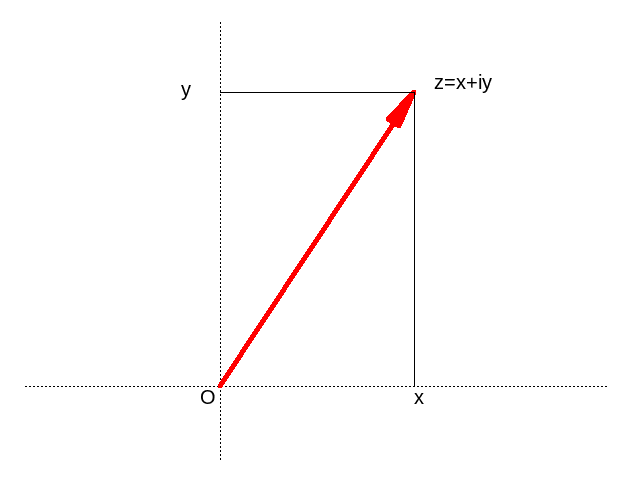
\includegraphics[width=0.7\linewidth]{chap1_01}
	\caption{复平面:每一个复数都与复平面上一个点相对应,与复数$z$对应的点也称作“点$z$”,$\vec{Oz}$与复数$z$一一对应。}
	\label{fig:chap1_01}
\end{figure}

\end{frame}

\begin{frame}{复数加法的几何意义}
\begin{figure}
	\centering
	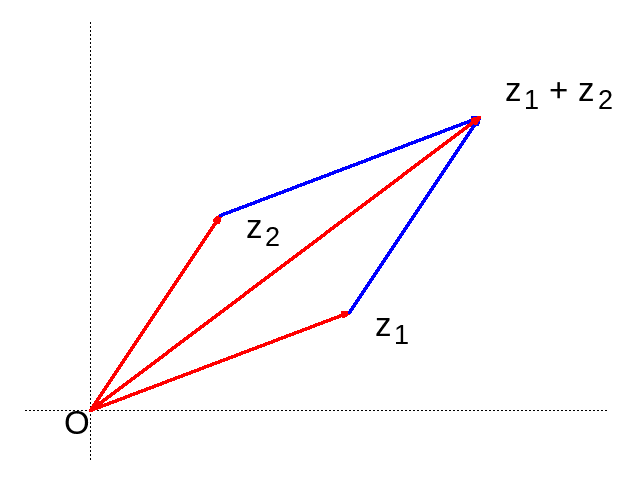
\includegraphics[width=0.7\linewidth]{chap1_02}
	\caption{复数加法对应着矢量相加。}
	\label{fig:chap102}
\end{figure}

\end{frame}

\begin{frame}{模与辐角}
模:原点$O$到$z$点的距离
\begin{equation}
r = |z| = \sqrt{x^2 + y^2},
\end{equation}
辐角:$x$轴正方向与$\vec{Oz}$的夹角(逆时针为辐角的正向),记作$Arg~z$。
辐角可以是多个值
\begin{equation}
Arg z = \theta + 2k \pi, k = 0, \pm 1, \pm 2, \cdots
\end{equation}
因为$x$轴正方向旋转这些角度都可以与$\vec{Oz}$重合。

\kong[0.5]

我们可以定义$[0,2\pi)$内的辐角为辐角主值,记作arg z,则有
\begin{equation}
Arg z = arg z + 2k\pi, k = 0, \pm 1, \pm 2, \cdots
\end{equation}
\end{frame}

\begin{frame}{极坐标}
二维平面上的一个点可以用直角坐标表示$(x,y)$,也可以用极坐标表示$(r,\theta)$,换算关系为
\begin{equation}
x = r \cos \theta, y = r \sin \theta,
\end{equation}
所以,复数$z$可以写作
\begin{equation}
z = x + iy = r\cos \theta + i r \sin \theta = r(\cos \theta + i \sin \theta).
\end{equation}
\end{frame}

\begin{frame}{欧拉公式}
利用泰勒展开公式,可以推出
\begin{eqnarray}
\cos \theta &=& 1 - \frac{1}{2}\theta^2 + \frac{1}{4!}\theta^4 - \frac{1}{6!}\theta^6 + \cdots, \\
\sin \theta &=& \theta - \frac{1}{3!}\theta^3 + \frac{1}{5!}\theta^5 + \cdots,
\end{eqnarray}
将这两个公式带入$\cos \theta + i \sin \theta$,会得到
\begin{equation}
\cos \theta + i \sin \theta = 1 + i\theta + \frac{1}{2}(i\theta)^2 + \frac{1}{3!}(i\theta)^3 + \cdots,
\end{equation}
而这正是$e^{i\theta}$的泰勒展开形式,所以
\begin{equation}
\cos \theta + i \sin \theta = e^{i\theta}.
\end{equation}
这就是欧拉公式。

\kong[0.5]

问:$e^{2\pi i} = ?$
\end{frame}

\begin{frame}{模与辐角}
有了欧拉公式,
\begin{equation}
z = r(\cos\theta + i\sin\theta) = r e^{i\theta}.
\end{equation}
这个形式清晰地体现了$z$在复平面上的几何性质:$r$是模,$\theta$是辐角。

\kong[0.5]

根据$e$指数的特点,有
\begin{eqnarray}
e^{i\theta_1} e^{i\theta_2} &=& e^{i(\theta_1 + \theta_2)},\\
e^{i\theta_1}/e^{i\theta_2} &=& e^{i(\theta_1 - \theta_2)},
\end{eqnarray}
\end{frame}

\begin{frame}{复数乘法的几何意义}
复数$z_1 = r_1 e^{i\theta_1}$与$z_2 = r_2 e^{i\theta_2}$的乘积为
\begin{equation}
z_1 z_2 = r_1 r_2 e^{i(\theta_1 + \theta_2)},
\end{equation}
所以,任意复数$z_1$乘以$z_2$以后,相当于$z_1$的模变为原来的$r_2$倍,辐角增加$\theta_2$。

\kong[0.5]

换一句话说,$\vec{Oz_1}$伸长/压缩$r_2$倍,并逆时针旋转$\theta_2$。

\end{frame}

\begin{frame}{例题}
分别写出下列复数的三角形式和指数形式
\begin{itemize}
	\item 1+i
	\item i
	\item 1
	\item -2
\end{itemize}
\end{frame}

\begin{frame}{乘幂}
因为
\begin{equation}
z = re^{i\theta},
\end{equation}
所以,$z$的$n$次幂可写作
\begin{equation}
z^n = (re^{i\theta})^n = r^n e^{in\theta} = r^n (\cos n\theta + i \sin n \theta),
\end{equation}
根据这个式子,可以推出所谓棣莫弗公式:
\begin{equation}
(\cos \theta + i \sin \theta)^n = \cos n\theta + i \sin n\theta,
\end{equation}
比如,可以轻易推出以下公式
\begin{eqnarray}
\cos 2\theta &=& \cos^2 \theta - \sin^2 \theta,\\
\sin 2 \theta &=& 2 \sin \theta \cos \theta.
\end{eqnarray}
\end{frame}

\begin{frame}{方根}
若要求$z$的$n$次方根,即求$\omega$,使得
\begin{equation}
\omega^n = z,
\end{equation}
把$\omega = \rho e^{i\varphi}, z = r e^{i\theta}$代入上式得到
\begin{equation}
\rho^n e^{in\varphi} = r e^{i\theta},
\end{equation}
所以有
\begin{equation}
\rho^n = r, n\varphi = \theta + 2k\pi,
\end{equation}
得到
\begin{equation}
\rho = r^{1/n}, \varphi = \frac{ \theta + 2k\pi }{n},
\end{equation}
其中$k=0,1,\cdots,n-1$,有$n$个不同的取值。
\end{frame}

\begin{frame}{例题}
用$\sin \theta, \cos \theta$表示出$\cos 3\theta, \sin 3\theta$。

\kong[0.5]

计算$(1+i)^{1/4}$的所有值
\end{frame}

\begin{frame}{邻域、内点、外点、孤立点}
$z_0$的邻域($\delta$邻域):
\begin{equation}
|z - z_0| < \delta,
\end{equation}
也记作$N_{\delta}(z_0)$,或$N(z_0)$。

\kong[0.5]

$z_0$的去心邻域:
\begin{equation}
0<|z - z_0| < \delta,
\end{equation}

\kong[0.5]
内点:若对平面点集$E$中点$z_0$,存在$N(z_0)$,该邻域内所有点都属于$E$,则称$z_0$是$E$的内点。

\kong[0.5]
外点:存在$N(z_0)$,该邻域内所有点都不属于$E$。

\kong[0.5]
边界点:对任意$N(z_0)$,有属于$E$的点,也有不属于$E$的点。

\kong[0.5]
孤立点:$z_0$属于$E$,但它的一个去心邻域都不属于$E$。

\end{frame}

\begin{frame}{内点、外点、边界点}
\pagecolor{blue}
\begin{figure}
	\centering
	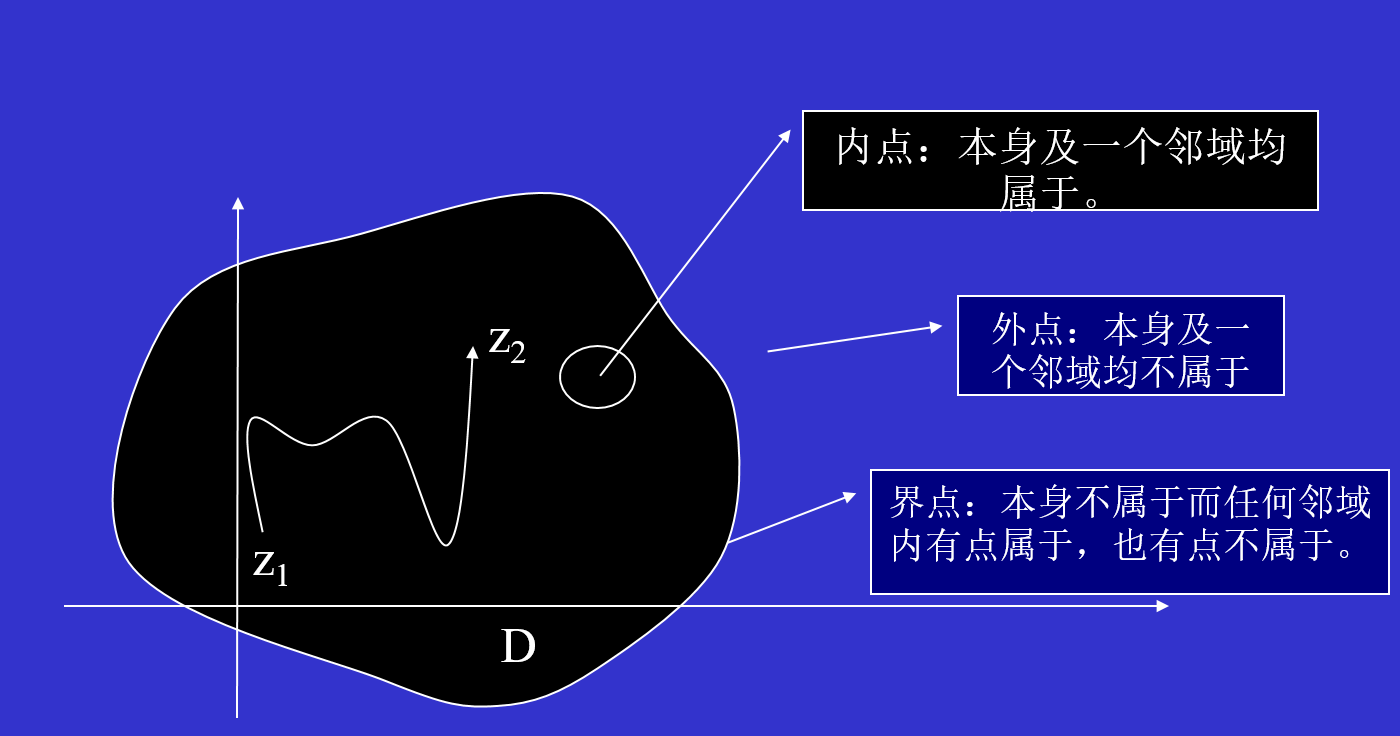
\includegraphics[width=0.9\linewidth]{chap1_03}
	\caption{内点、外点、边界点。}
	\label{fig:chap103}
\end{figure}

\end{frame}

\begin{frame}{区域、闭区域}
\kong[0.5]
开集:$E$内所有点都是内点。

\kong[0.5]
连通:$E$内任意两个点都可以用一条内部的曲线连接

\kong[0.5]
{\color{blue}区域:连通的开集}

\kong[0.5]
闭区域:区域$D$+它的边界 = 闭区域$\bar{D}$

\kong[0.5]
区域边界的正方向:区域内所有点都在左边

\end{frame}

\begin{frame}{曲线}
连续曲线:
\begin{equation}
z(t) = x(t) + iy(t),
\end{equation}
其中$x(t),y(t)$是连续实函数,$\alpha \leq t \leq \beta$。

\kong[0.5]
重点:若对$t_1 \neq t_2$(不同时为区间端点),有$z(t_1) = z(t_2)$,则$z(t_1)$为曲线重点。

\kong[0.5]
简单曲线(若尔当曲线):没有重点

\kong[0.5]
简单闭曲线:没有重点,且$z(\alpha)=z(\beta)$

\kong[0.5]
光滑曲线:$x'(t), y'(t)$在$[\alpha, \beta]$上存在且不同时为零。

\kong[0.5]
逐段光滑曲线:由有线条光滑曲线衔接而成

\kong[0.5]
单连通域:区域$D$内任一条简单闭曲线都可以不经过$D$的边界,而收缩为$D$内的点。否则称作复连通域。
\end{frame}

\begin{frame}{区域、曲线}
\begin{figure}
	\centering
	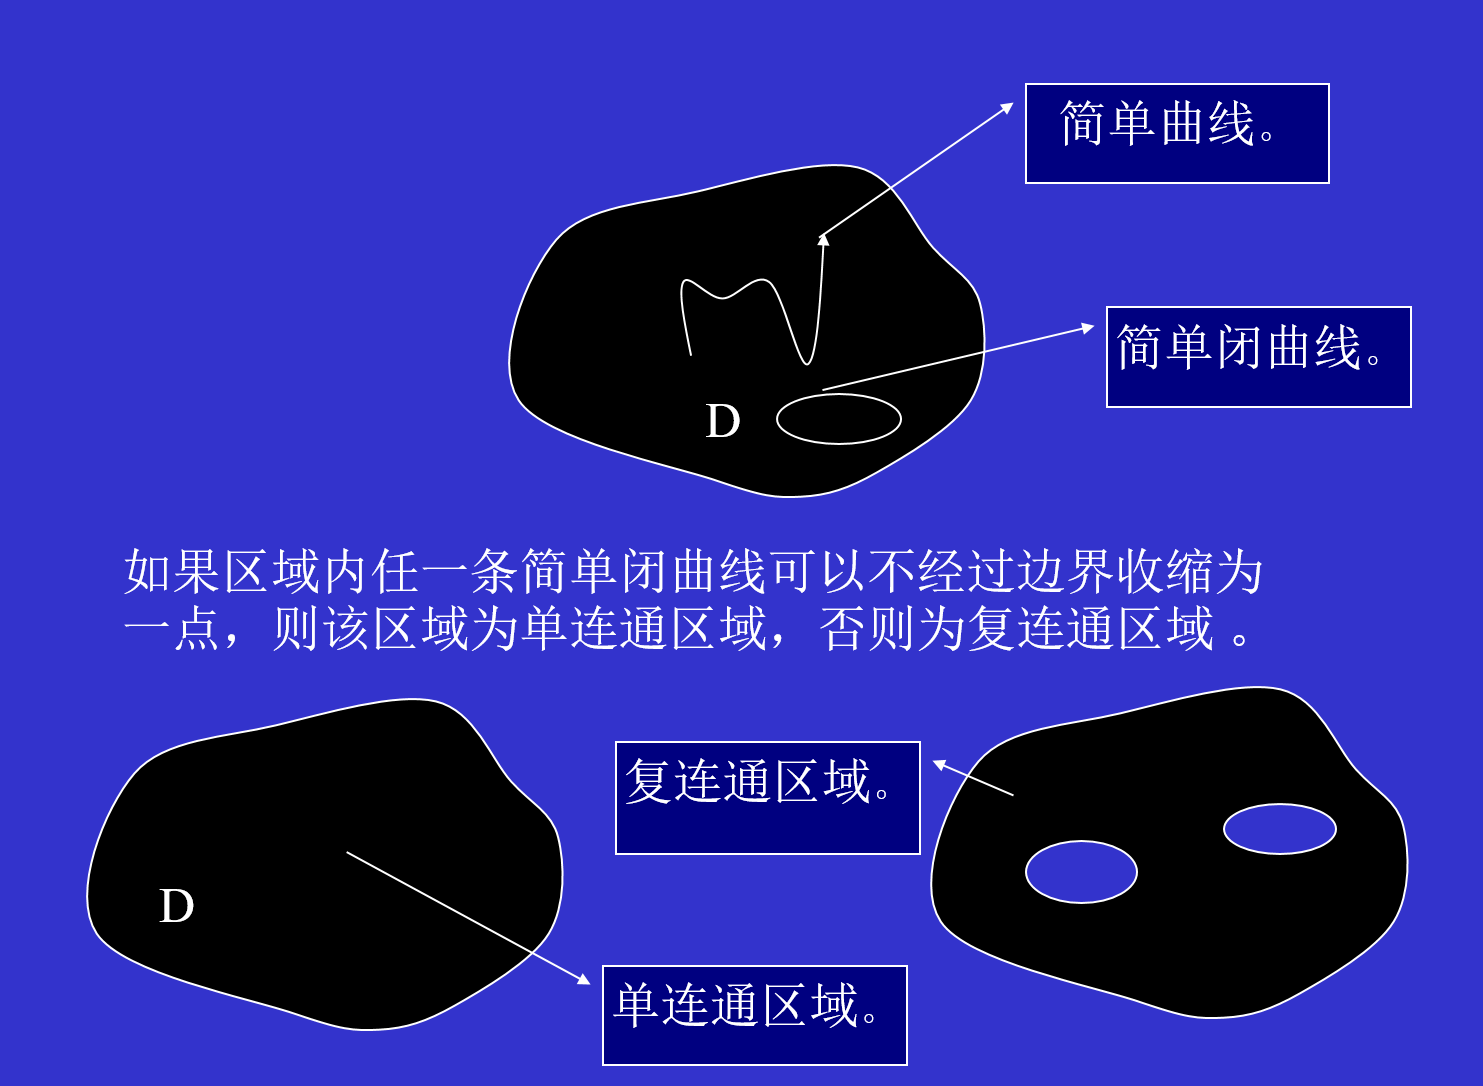
\includegraphics[width=0.7\linewidth]{chap1_04}
	\caption{简单曲线、单连通区域、复连通区域}
	\label{fig:chap104}
\end{figure}

\end{frame}

\begin{frame}{简单曲线、区域}
\begin{figure}
	\centering
	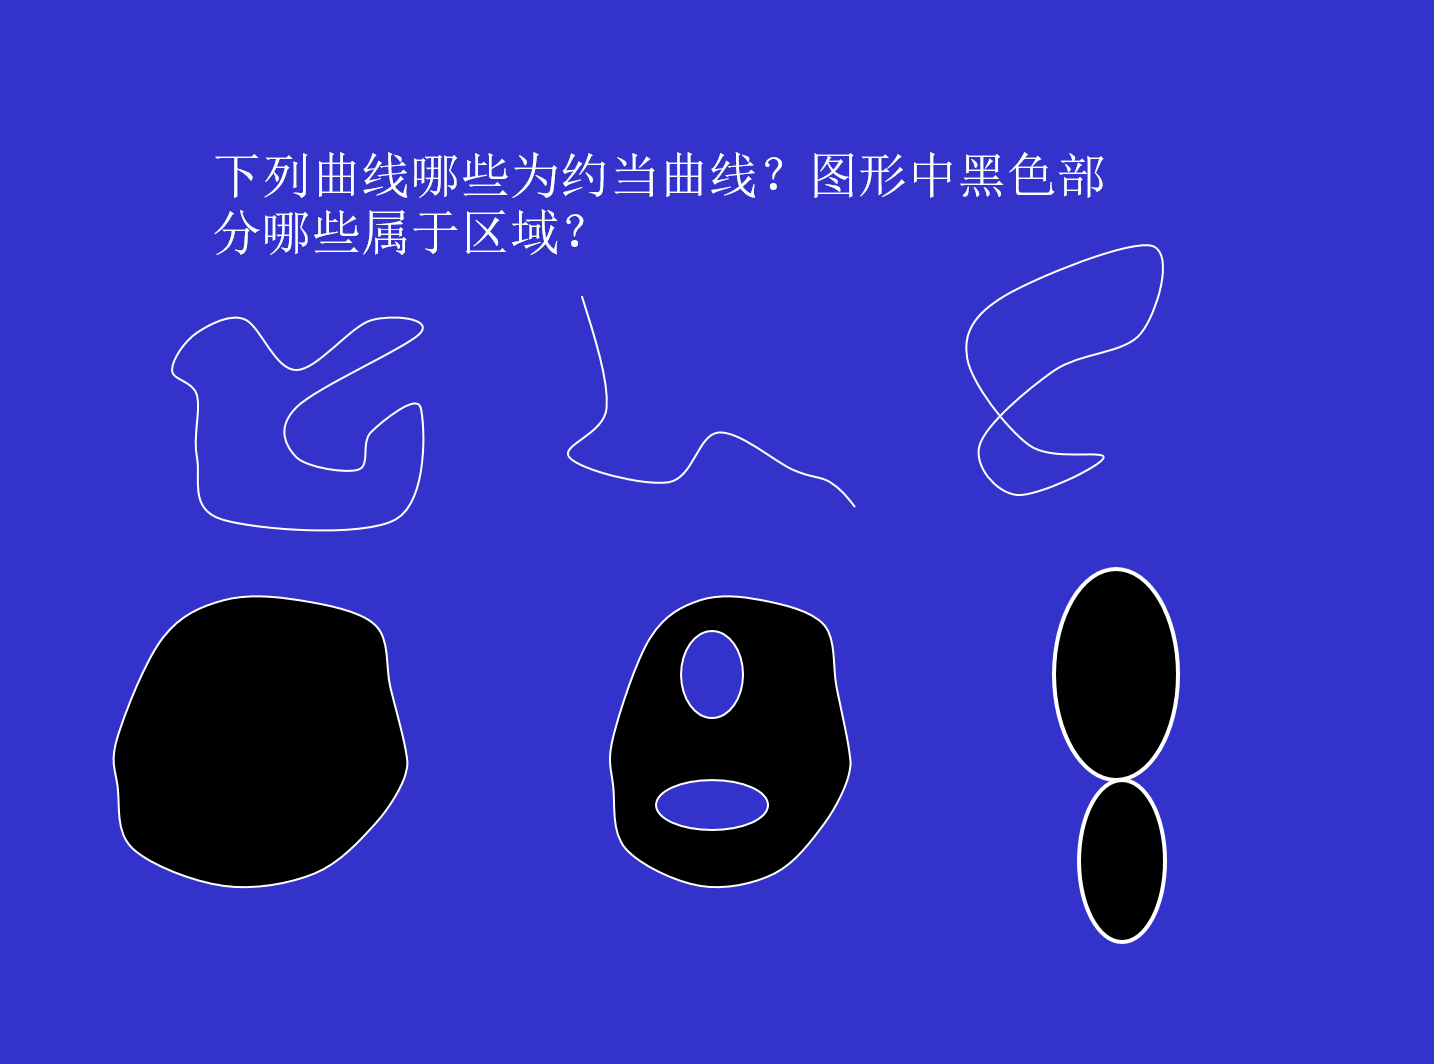
\includegraphics[width=0.7\linewidth]{chap1_05}
	\label{fig:chap105}
\end{figure}
\end{frame}

\begin{frame}{区域的复数表达}
\begin{figure}
	\centering
	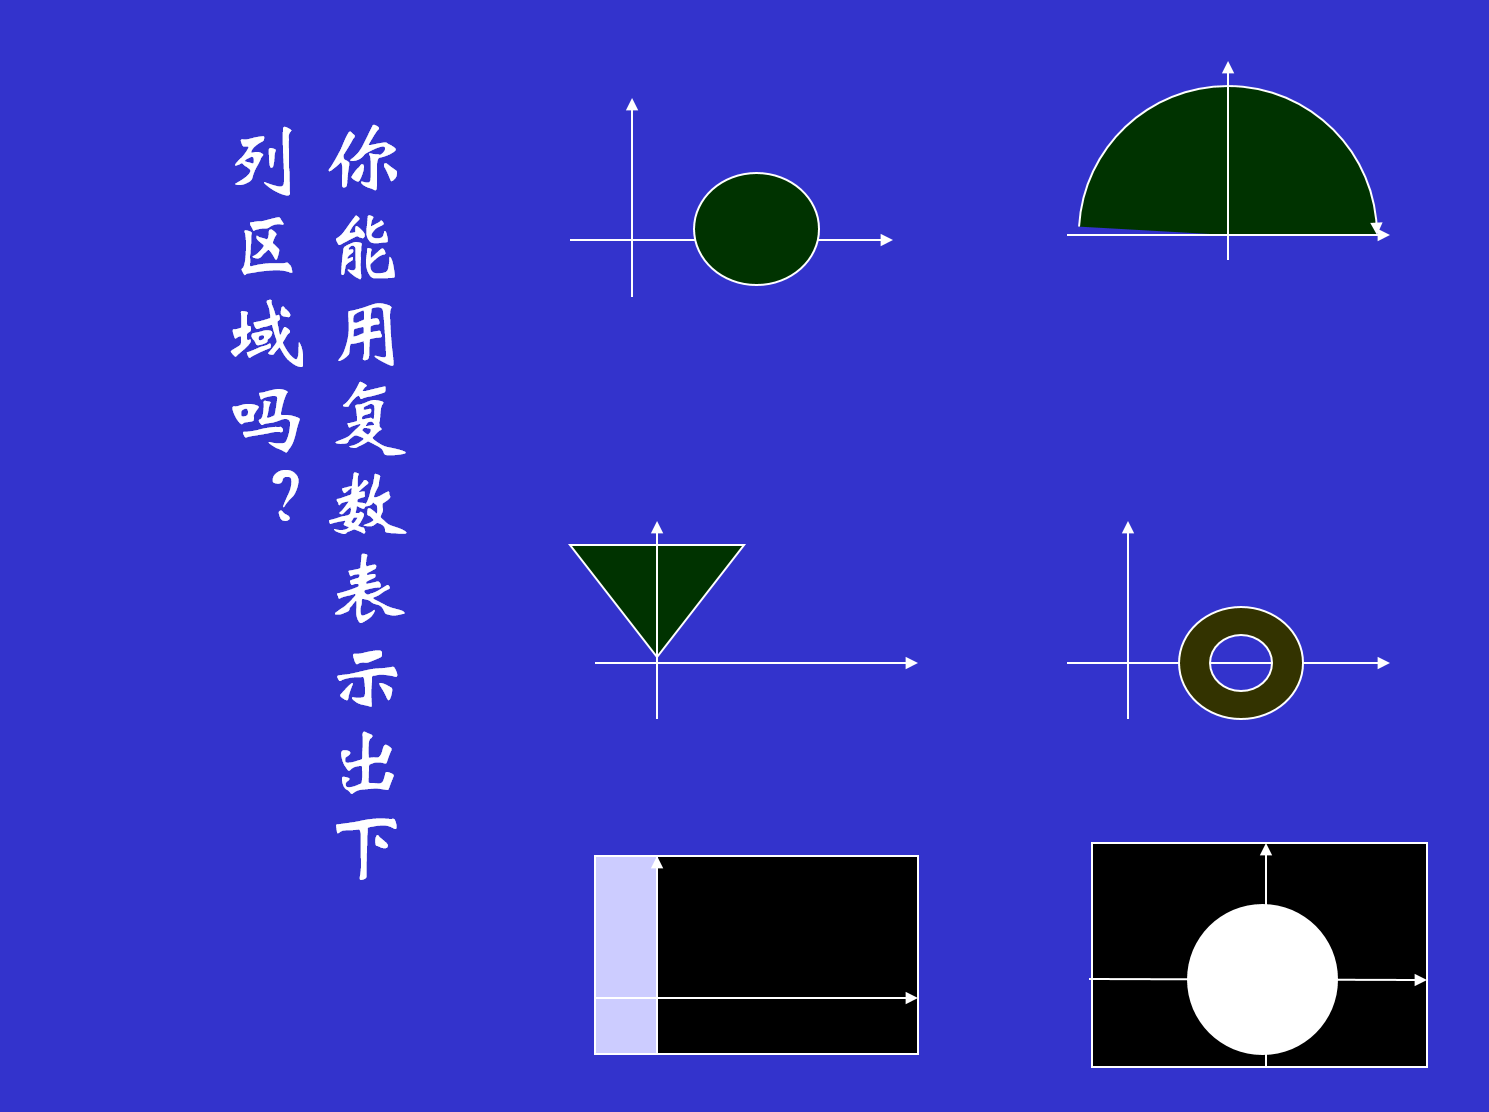
\includegraphics[width=0.7\linewidth]{chap1_06}
	\label{fig:chap106}
\end{figure}
\end{frame}

\begin{frame}{复变函数}
\begin{equation}
\omega = f(z),z \in E,
\end{equation}
其中$E$是一个复数集。

\kong[0.5]
单值函数:$z$对应唯一的$\omega$。否则称为多值函数。今后若不特别声明,所提到的函数都指单值函数。

\kong[0.5]
单叶函数:若$z_1 \neq z_2$,必有$f(z_1) \neq f(z_2)$

\kong[0.5]
$\omega$与$z$通过$\omega = f(z)$联系,可看作是$z$平面与$\omega$平面之间的映射。
\end{frame}

\begin{frame}{复变函数的极限与连续性}
极限:对任意$\epsilon>0$,都存在$\delta>0$,使得$N_\delta(z_0)$内有
\begin{equation}
|f(z) - \omega_0 | < \epsilon,
\end{equation}
则说$f(z)$在$z\rightarrow z_0$时趋于$\omega_0$,记作
\begin{equation}
\lim\limits_{z \rightarrow z_0} f(z) = \omega_0.
\end{equation}

\kong[0.5]
连续性:对任意$\epsilon>0$,都存在$\delta>0$,使得$N_\delta(z_0)$内有
\begin{equation}
|f(z) - f(z_0)| < \epsilon,
\end{equation}
则称$f(z)$在$z=z_0$连续。

\kong[0.5]
这与实函数的极限、连续性定义是一样的。
\end{frame}

\begin{frame}{映射、极限}
\begin{figure}
	\centering
	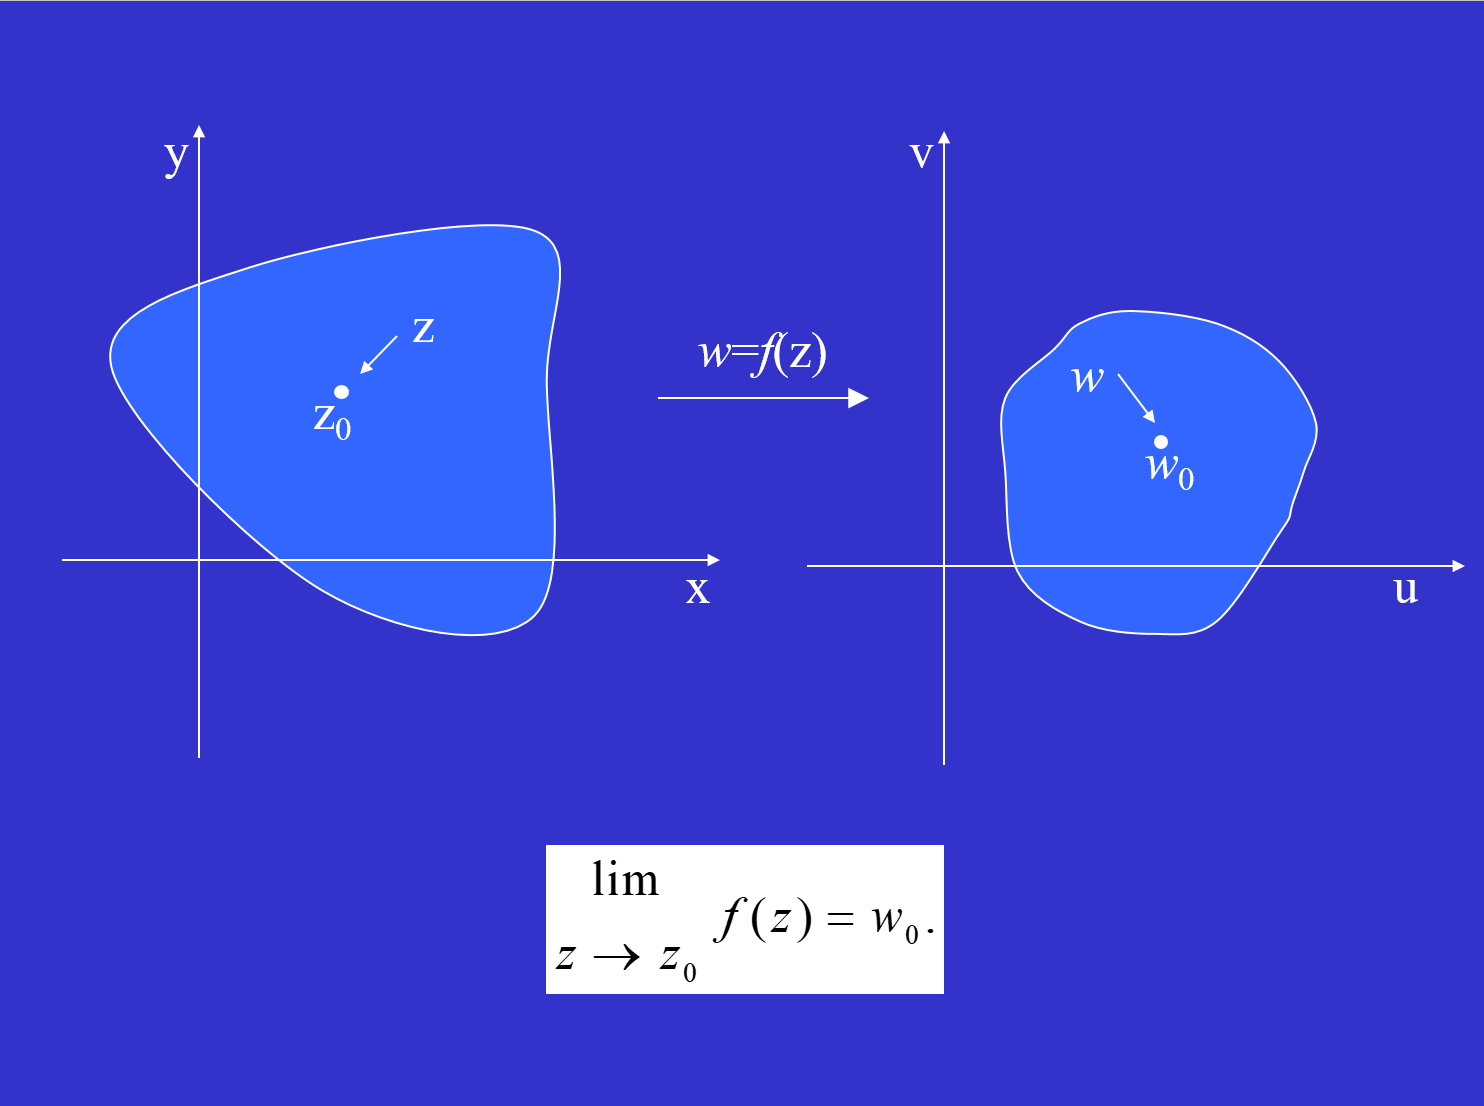
\includegraphics[width=0.7\linewidth]{chap1_07}
	\caption{复变函数:两个复数域之间的映射;复变函数的极限。}
	\label{fig:chap107}
\end{figure}

\end{frame}

\begin{frame}{复变函数的连续性}
\begin{equation}
f(z) = u(x,y) + iv(x,y)
\end{equation}
在$z_0 = x_0 + i y_0$连续的充要条件是$u(x,y), v(x,y)$在$x_0, y_0$连续。

\kong[0.5]
若$f(z)$在有界区域$\bar{D}$上连续,则有
\begin{itemize}
	\item 在$\bar{D}$上$f(z)$有界,即$|f(z)|$在$\bar{D}$上有界
	\item $|f(z)|$在$\bar{D}$上有最大值和最小值
	\item $f(z)$在$\bar{D}$上一致连续,即对任意$\epsilon>0$,存在$\delta>0$,使得$\bar{D}$上对任意满足$|z_1 - z_2|<\delta$的$z_1,z_2$,有$|f(z_1)-f(z_2)|<\epsilon$。
\end{itemize}
\end{frame}

\begin{frame}{复球面}
\begin{figure}
	\centering
	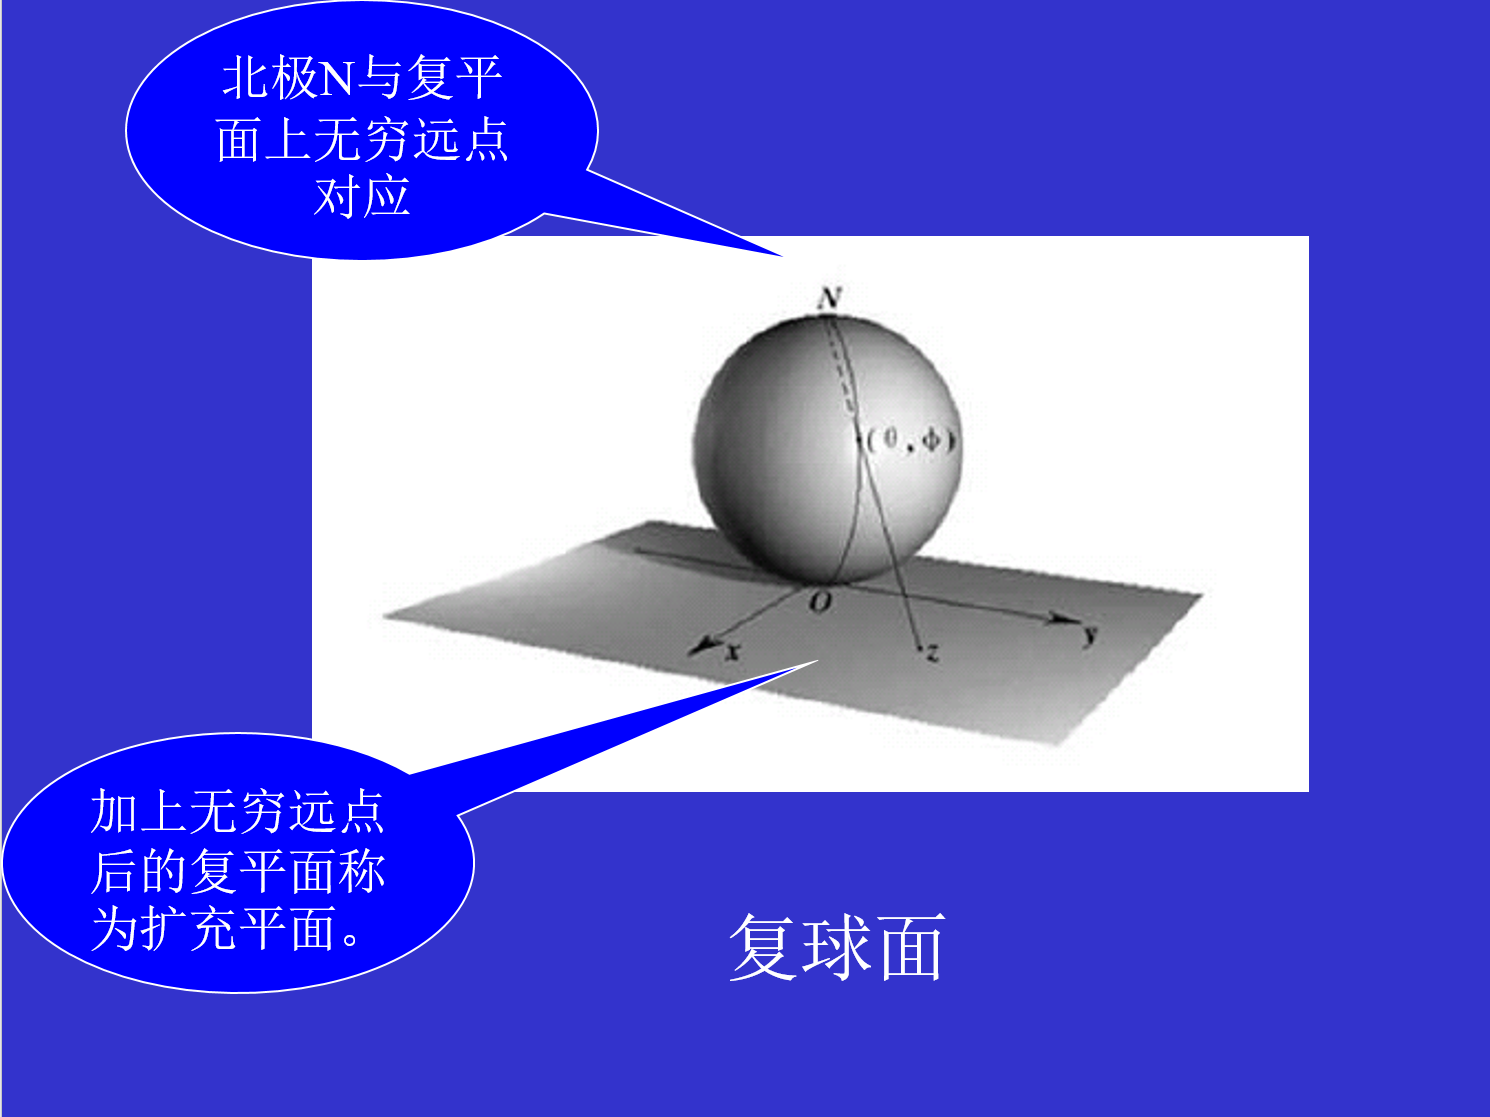
\includegraphics[width=0.6\linewidth]{chap1_08}
	\caption{复球面与复平面之间的一一对应。}
	\label{fig:chap108}
	
	另外:$z=\infty$的$\epsilon$-邻域$N_\epsilon(\infty): |z| > 1/ \epsilon $。
\end{figure}

\end{frame}

\begin{frame}{练习}
\kong[0.5]

课堂讲解:习题1, 4, 8, 11, 16

\kong[0.5]

课下练习:习题2, 3, 5, 9, 10
\end{frame}

\end{document}
